We describe a realistic setting where we can obtain small, in average, HL for the CSP.

First, we assume that individual edges are shortest paths, which is clearly true in road networks, and add an additional constraint wherein we insist our efficient paths have bounded \emph{stretch} compared to the shortest path; note that this is natural in applications as users do not want to be presented solutions which are far away from the optimum, even if it saves them budget.
Formally, we define:

\begin{definition}[Stretch]
	An algorithm for CSP has stretch $\St\geq 1$ if, $\forall s,t\in V$ and $b\leq B$, outputs $\dist(s,t|b)$ whenever $\dist(s,t|b)\leq \St\dist(s,t)$ and outputs ``infeasible'' when $\dist(s,t|b)>\St\dist(s,t)$.
\end{definition}
We henceforth input $\St$ as an extra constraint given by the application. 
Next, let $\Ec\defeq\crl{e\in E:c_e>0}$ denote the set of `costly' edges.
We define the following notion of an \emph{overpass}:

\begin{definition}[Overpass]
For $r>0$, the edge $e=(u,v)$ is an $r$-overpass if:\\
$(1)$ $e$ belongs to a path $Q\in\PE_{2r}\setminus\PS$\\
$(2)$ both $u$ and $v$ are endpoints of paths in $\PS_{r(2/\St-1)}$ and\\ 
$(3)$ $\min(\dist(e,\Ec),\dist(\Ec,e))\leq 3r/2$
\end{definition} 
Essentially, overpasses are edges connecting long shortest-paths in a costly zone; \cref{fig:overpass} shows an example. In case costs are contiguous (for example, tolls on highways or traffic jams), then the definition corresponds to the intuitive notion of an overpass.
Our main requirement is the following \emph{bounded growth} condition, controlling the number of $r$-overpasses for every scale $r>0$.

\begin{figure}[!b]
	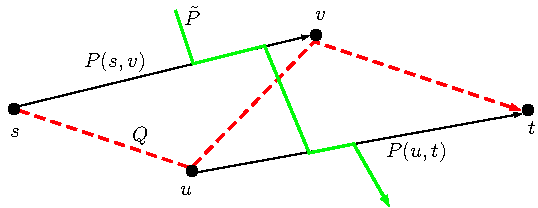
\includegraphics[scale=0.6]{TexImg/overpass.pdf}
	\caption{Edge $uv$ here is an overpass, lying on efficient path $Q$ (dashed red), connecting a pair of long shortest paths $P(s,v)$ and $P(u,t)$, and close to costly edges $\tilde P$ (solid green). } 
	\label{fig:overpass}
\end{figure}


\begin{definition}[Bounded Growth]
$(G,c,\ell)$ satisfies the bounded growth condition if, $\forall r>0$, $\abs{\crl{u\in V: \exists v, uv \text{ is an $r$-overpass}}}\leq \phi(2r)$, where $\phi(r)\defeq nh\alpha^{\beta-2-\log_2r}$
\end{definition}

Observe that $\phi$ is a slowly decreasing function of $r$ and, even when $r=D$, we allow for overpasses.
Now, with these conditions, we get our main result of this section:


\begin{theorem}\label{theo:overpasses}
Let $(G,\ell,c)$ be a network with HD $h$.
If the bounded growth is satisfied, we can obtain, in polynomial time, hub labels for CSP queries that guarantee average query-time $\Or((b+1)\alpha h'\log D)$ and total storage $\Or(nB\cdot B\alpha h'\log D)$, where $h'=\Or(\Delta h\log(hn\Delta))$.
\end{theorem}

We henceforth refer to the average HD of $\PE$ as average CHD; since the average HD is enough to obtain good preprocessing algorithms (cf. \cref{theo:preproc_avg}), an average CHD should intuitively suffice.
However, to prove \cref{theo:overpasses}, we need to show that it is possible to obtain small average CHD under even less restrictive assumptions than the partial-witness.
To do this, we first allow for an additional \emph{supplementary witness set} $D$ such that \emph{every efficient path is either witnessed by a shortest-path or hit by $D$}.
This corresponds to the intuition that a few bad efficient paths should not completely ruin the algorithm. 

\begin{definition}[Weak Partial Witness]
Given $\beta\geq 0$, we say a path system  $\calQ$ is weakly $\beta$-witnessed by the path system $\calQ'$ if, for every $r>0$, $\exists D_r\subseteq V$ such that, $\forall Q\in \calQ_r$ either (1) $Q$ is $\beta$-witnessed by $\calQ'$ or (2) $Q$ is hit by $D_r$.
Additionally we require $\abs{D_r}\leq \phi(r)$.
\end{definition} 

Intuitively, the supplementary witness set $D_r$ takes care of all the corner cases where $\calQ$ and $\calQ'$ differ too much.
We now show that our requirement on $\abs{D_r}$ guarantees a bound on the average HD.

\begin{proposition}\label[proposition]{prop:lay_witness}
Assume that $G$ is $\alpha$-doubling and let $\calQ'$ be weakly $\beta$-witnessed by $\calQ$.
If the HD of $\calQ$ is $h$, then the average HD of $\calQ'$ is $h'\leq 2\alpha^{\beta}h$
\end{proposition}
\begin{proof}
Let $r>0$, and $C$ be an $(h,2^{-\beta}r)$-LSHS for $\calQ$.
We show that $C\cup D_r$ is an average $(h,r)$-LSHS for $\calQ'$.
Clearly is a hitting set for $\calQ'_r$ and we can compute
\begin{align*}
h'&\leq \frac{1}{n}\sum_{v\in V} \abs{B_{2r}(v)\cap (C\cup D_r)}\\
&\leq \frac{1}{n}\prn*{\sum_{v\in V} \abs{B_{2r}(v)\cap C}+\sum_{v\in V} \abs{B_{2r}(v)\cap D_r}}\\
&\leq \frac{1}{n}\prn*{\sum_{v\in V} \alpha^\beta h+\sum_{v\in D_r} \abs{B_{2r}(v)}}
\leq \alpha^\beta h + \frac{\abs{D_r}\alpha^{\log_2r+2}}{n}.
\end{align*}
In the third inequality we used that $C$ is sparse with respect to balls of radius $2^{-\beta+1}r$ and that $\sum_{v\in V} \abs{B_{2r}(v)\cap D_r}=\sum_{v\in D_r} \abs{B_{2r}(v)}$ by symmetry of the bi-directional balls.
In the last inequality we used that, by doubling dimension, balls of radius $r$ have at most $\alpha^{\log_2r+1}$ elements.
Since $\abs{D_r}\leq \phi(r)$, the result follows.
\end{proof}

This now allows us to link $\PE$ and $\PS$ as follows:
\begin{proposition}\label[proposition]{prop:1witness}
Under the bounded growth condition, $\PS$ is a weak $1$-witness for $\PE$.
\end{proposition}
\begin{proof}
We first need some additional notation:
For a path $Q$ and two vertices $u,v\in Q$ we denote $Q[u,v]\subseteq Q$ as the sub $(u,v)$-path; for two paths $P,Q$ with a common endpoint, we denote $P|Q$ as their concatenation.

Consider $Q\in\PE$ with endpoints $s,t$ and set $\ell(Q)=2r$.
We will show how to obtain a vertex for the supplementary witness set in case $Q$ is not witnessed and then we bound the size of the set.
Assume that $Q\neq P(s,t)$, otherwise the path is trivially witnessed.
Let $(u,v)\in Q$ be such that $\ell(Q[s,v]),\ell(Q[u,t])\geq r$. 
If either $Q[s,v]$ or $Q[u,t]$ is a shortest path or $\ell_{uv}\geq r$, then $Q$ is witnessed. Thus, we henceforth assume that all of the above conditions fail.

We claim that $uv$ is a $r$-overpass (in fact, this is the exact scenario depicted in \cref{fig:overpass}).
Condition 1 is clearly satisfied. 
Condition 2 also holds because both $Q[s,v]$ or $Q[u,t]$ have stretch at most $\frac{2-\St}{\St}$.
To see this, note that both $P(s,v)|Q[v,t]$ and $Q[s,u]|P(u,t)$ are no shorter than $P(s,t)$ and $\St\ell(P(s,t))\geq \ell(Q)$, hence
$\frac{2r}{\St}\leq \ell(P(s,t)) \leq  \ell(P(s,v)) + \ell(Q[v,t])$ and $\frac{2r}{\St} \leq \ell(P(s,t)) \leq  \ell(Q[s,u]) + \ell(P(u,t))$.
Since each path $Q[s,u],Q[v,t]$ has length less than $r$, it follows that both $P(s,v),P(u,t)$ have length strictly greater than $\frac{2-\St}{\St}r$. % and condition 1 follows. 
Finally, to show condition 3, we have $\ell(Q[s,v])+\ell(Q[u,t])=r+\ell_{uv}$ and since $\ell_{uv}<r/2$, one of $Q[s,v]$ or $Q[u,t]$ has length at most $3r/4$.
Since neither of these paths is shortest, it must be that both $P(s,v),P(u,t)$ have costly edges and thus one of $u,v$ is closer than $3r/4$ to $E_1$ and the condition is satisfied.

For every path of length $2r$, we can thus either exhibit a witness or show that it contains an overpass and add use the tail of the edge as a supplementary witness.
For a fixed $r>0$, we need to add at most $\phi(r)$ nodes to $D_r$ to cover all the efficient paths. 
The result follows.
\end{proof}

We are almost ready to prove that bounded growth allows to solve the CSP.
The last piece is \cref{prop:avg_chd}, the proof of which follows form similar arguments as those in \cref{theo:HLeff,theo:preproc_avg}.

\begin{proposition}\label[proposition]{prop:avg_chd}
If the average HD of $\PE$ is $h_c$, then we can construct, in polynomial time, hub labels for CSP, which guarantee average query-time $\Or((b+1)h_c'\log D)$ for queries with budget $b$, and total storage requirements $\Or(nB\cdot Bh_c'\log D)$.
\end{proposition}

\begin{proofof}{\cref{theo:overpasses}}
We argue that the average CHD is $h_c\leq 2\alpha h$.
By \cref{prop:1witness}, $\PE$ is weakly $1$-witnessed by $\PS$.
It follows by \cref{prop:lay_witness} that the average CHD is at most $2\alpha h$ as needed.
Applying \cref{prop:avg_chd} yields the result.
\end{proofof}